\section{Sensitivity and Reliability}
\subsection{Transaction-cost stress with the policy frozen}
The saved final cost sweep changes the fee rate while keeping the strategic model and customer assignments fixed. The cost gate still responds to the fee it faces. Table~\ref{tab:cost} and Figure~\ref{fig:cost} therefore describe a fixed decision rule under different execution costs, not a refitted strategy.

\begin{table}[h!]
\centering
\caption{Thirty-year Balanced A under alternative transaction costs. Growth and drawdown are in \%; fees are real wealth units.}
\label{tab:cost}
\begin{tabular}{rrrrrr}\toprule
Cost (\%) & Med. $G$ & P10 $G$ & P90 $D$ & Mean fees & Trades (\%)\\\midrule
\tableinput{generated/costs.tex}
\bottomrule\end{tabular}
\end{table}

\begin{figure}[h!]
\centering
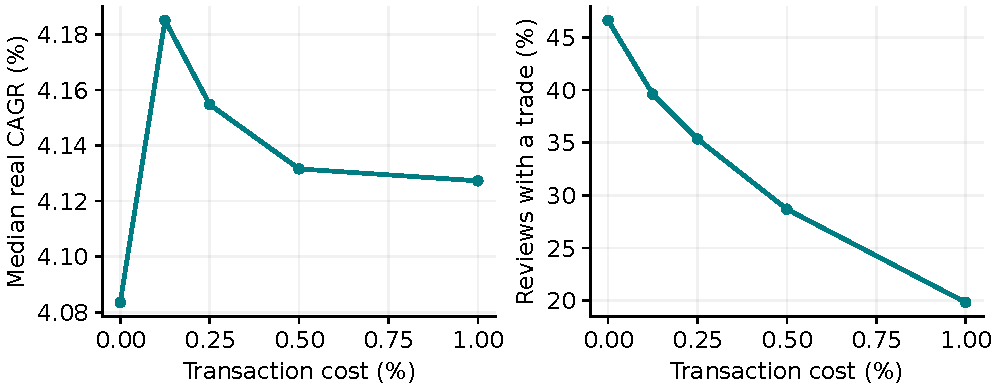
\includegraphics[width=\linewidth]{figures/cost_sensitivity.pdf}
\caption{Higher fees suppress trading; growth need not fall monotonically because the actions also change.}
\label{fig:cost}
\end{figure}

Doubling the fee to 0.50\% reduces the trading rate to \DoubleTrades\%, while median real growth remains \DoubleGrowth\%. Mean real fees rise to \DoubleCost{}. Small nonmonotonic growth differences should not be interpreted as a benefit from charging fees: changed trades lead to changed exposures on the same finite set of scenarios.
